% Copyright (c) 2026 Islam Ibrahim. All rights reserved.

\documentclass[tikz,border=10pt]{standalone}
\usepackage[T1]{fontenc}
\usepackage{lmodern}
\usepackage{amsmath}
\usepackage{tikz}
\usetikzlibrary{arrows.meta,positioning,fit,backgrounds}

\definecolor{matlabCol}{HTML}{D97824}
\definecolor{fdtdCol}{HTML}{2E86C1}
\definecolor{deviceCol}{HTML}{249B5B}
\definecolor{interCol}{HTML}{7D3C98}

\begin{document}
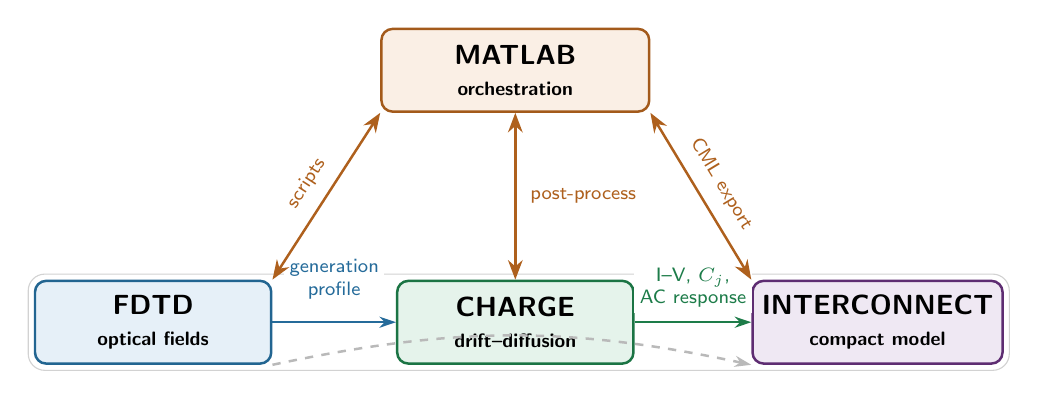
\begin{tikzpicture}[font=\small\sffamily,>=Stealth,
  box/.style={draw=#1!75!black,fill=#1!12,line width=0.9pt,
    rounded corners=4pt,minimum width=3.0cm,minimum height=1.05cm,
    align=center,font=\bfseries\sffamily},
  data/.style={-{Stealth[length=6pt,width=4pt]},line width=0.9pt,#1},
  label/.style={font=\scriptsize\sffamily,align=center,fill=white,inner sep=2pt},
]

\node[box=matlabCol,minimum width=3.4cm] (matlab) at (0,3.2) {MATLAB\\[-1pt]\scriptsize orchestration};
\node[box=fdtdCol] (fdtd) at (-4.6,0) {FDTD\\[-1pt]\scriptsize optical fields};
\node[box=deviceCol] (device) at (0,0) {CHARGE\\[-1pt]\scriptsize drift--diffusion};
\node[box=interCol] (inter) at (4.6,0) {INTERCONNECT\\[-1pt]\scriptsize compact model};

\draw[data=fdtdCol!80!black] (fdtd) -- node[label,above=6pt] {generation\\profile} (device);
\draw[data=deviceCol!80!black] (device) -- node[label,above=3pt] {I--V, $C_j$,\\AC response} (inter);

\draw[data=matlabCol!80!black,<->] (matlab.south west) -- node[label,sloped,above=3pt] {scripts} (fdtd.north east);
\draw[data=matlabCol!80!black,<->] (matlab.south) -- node[label,right=3pt] {post-process} (device.north);
\draw[data=matlabCol!80!black,<->] (matlab.south east) -- node[label,sloped,above=3pt] {CML export} (inter.north west);

\draw[data=gray!55,dashed,bend left=12] (fdtd.south east) to (inter.south west);

\begin{scope}[on background layer]
  \node[draw=gray!35,fill=gray!6,rounded corners=6pt,
    fit=(fdtd)(device)(inter),inner xsep=13pt,inner ysep=12pt,
    label={[font=\scriptsize\sffamily,gray!65]below:solver chain}] {};
\end{scope}

\end{tikzpicture}
\end{document}
